\documentclass[12pt]{article}
\usepackage{graphicx}
\usepackage{hyperref}
\title{Testing Policy}
\author{Binary Ninjaz}
\date{}

\hypersetup{
	colorlinks=true,
	linkcolor=black,
	filecolor=magenta,
	urlcolor=cyan,
}



% define the title
\author{Binary Ninjaz}
\title{Harvest}
\begin{document}
\begin{titlepage}

	\begin{center}
		% Upper part of the page
		\textsc{\LARGE Binary Ninjaz}\\[0.3cm]
		% Title
		\rule{\linewidth}{0.5mm} \\[0.5cm]
		{ \huge \bfseries Harvest \\
		  \vspace{0.3cm}\large \bfseries User Manual}\\[0.5cm]
		\rule{\linewidth}{0.5mm} \\[1cm]


		\begin{minipage}{0.4\textwidth}
			\begin{flushleft} \large
				\emph{} \\
				Letanyan {Arumugam}
			\end{flushleft}
		\end{minipage}
		\begin{minipage}{0.4\textwidth}
			\begin{flushright} \large
				\emph{} \\
				14228123
			\end{flushright}
		\end{minipage}

		\begin{minipage}{0.4\textwidth}
			\begin{flushleft} \large
            	\emph{} \\
				Sizo {Duma}
			\end{flushleft}
		\end{minipage}
		\begin{minipage}{0.4\textwidth}
			\begin{flushright} \large
				\emph{} \\
				15245579
			\end{flushright}
		\end{minipage}

		\begin{minipage}{0.4\textwidth}
			\begin{flushleft} \large
				\emph{} \\
				Teboho {Mokoena}
			\end{flushleft}
		\end{minipage}
		\begin{minipage}{0.4\textwidth}
			\begin{flushright} \large
				\emph{} \\
				14415888
			\end{flushright}
		\end{minipage}

		\begin{minipage}{0.4\textwidth}
			\begin{flushleft} \large
				\emph{} \\
				John {Ojo}
			\end{flushleft}
		\end{minipage}
		\begin{minipage}{0.4\textwidth}
			\begin{flushright} \large
				\emph{} \\
				15096794
			\end{flushright}
		\end{minipage}

        \begin{minipage}{0.4\textwidth}
			\begin{flushleft} \large
				\emph{} \\
				Kevin {Reid}
			\end{flushleft}
		\end{minipage}
		\begin{minipage}{0.4\textwidth}
			\begin{flushright} \large
				\emph{} \\
				15008739
			\end{flushright}
		\end{minipage}
        
        \begin{minipage}{0.4\textwidth}
			\begin{flushleft} \large
				\emph{} \\
				Shaun {Yates}
			\end{flushleft}
		\end{minipage}
		\begin{minipage}{0.4\textwidth}
			\begin{flushright} \large
				\emph{} \\
				16007493
			\end{flushright}
		\end{minipage}

		\vspace{1cm}
		\rule{\linewidth}{0.5mm} \\[1cm]
		\textsc{\Large Stakeholders}\\[1cm]

		\begin{minipage}{0.4\textwidth}
			\begin{flushleft} \large
				\emph{} \\
				SAMAC:
			\end{flushleft}
		\end{minipage}
		\begin{minipage}{0.4\textwidth}
			\begin{flushright} \large
				\emph{} \\
				Barry Christie
			\end{flushright}
		\end{minipage}


	\end{center}
\end{titlepage}

\newpage
\pagenumbering{Roman}
\tableofcontents
\newpage
\listoffigures

\newpage
\pagenumbering{arabic}
  
%\section{Introduction}
%Automated testing is vital in ensuring the number of defects in a program is as limited as possible. While having automated testing does not guarantee an absence of defects in a program it can greatly reduce that number; furthermore it serves to continually test and verify the function of modules that may be changed or affected upon by other changes.\\
%\indent While Binary Ninjaz intends to have as comprehensive test suite, they will not accept that wholly passing test cases means that a program is without flaw.\\
%\indent This document details the testing policies that are used by Binary Ninjaz in order to guide development and ensure a quality product; the specific testing methods used, and their impact of their effects on the general development process is described.

\section{Testing Process}
In this section, the testing process, based on IEEE-829, will illustrated. This process will fulfil the requirements stated in this document.\\
\indent Three phases within the testing process can be identified, namely:
\begin{enumerate}
	\item Test specification,
	\item Test implementation, and
	\item Test reporting.
\end{enumerate}
Each phase is now elaborated.
\subsection{Test specification}
The test specification can be subdivided into 2 parts. On the one hand, there is \textit{planning and verification}, on the other there is \textit{Analysis, design, and implementation}.\\
\indent \textit{Planning and verification} may consist of the following activities:\\
\begin{itemize}
 \item Specifying the scope and the risks, and defining the objectives of the tests;
\item Determining the strategy;
\item Taking decisions with regard to what must be tested, what roles apply, how the test activities will take place and how the outcomes of the tests will be implemented;
\item Planning of the test design activities;
\item Planning of implementation and evaluation.
\end{itemize}
During the \textit{analysis, design, and implementation} phase, the test objectives will be transformed into specific test conditions and test cases. This may involve the following activities: \newline
\begin{itemize}
 \item A review of the test base (such as requirements, architecture, design, and interfaces);
\item Evaluation of the testability of the test base and the test objects;
\item Identification and prioritisation of the test conditions;
\item Designing of the test cases;
\item Identifying the necessary test data in order to support the test cases;
\item Designing the test environment and identifying the infrastructure and tools.
\end{itemize}
\subsection{Implementation of tests}
The implementation of tests forms the phase in which the test procedures and scripts are implemented and the results of these (including incidents) are logged. This may involve the following activities: \newline
\begin{itemize}
 \item Implementation of the tests, manually or by means of a tool  
\item Logging the results of the implementation 
\item Comparing the results with the result that had been predicted 
\item Reporting any setbacks in the form of incidents and analysing these in order to identify the cause 
\item Repeating the tests as a result of the incidents identified 
\end{itemize}
\subsection{Test Reporting}
Test Reporting forms the phase in which the implementation of the tests is compared with the objectives. This may involve the following tasks: \newline
\begin{itemize}
 \item Checking of the test logs and the list of defects and comparing these to the exit criteria specified in the test plan   
\item Investigating whether additional tests are required
\item Writing a summary report 
\end{itemize}

  \section{TESTING TOOLS - unit testing level}
Unit tests (otherwise known as component tests) seek to identify defects in, and verify the functioning of, testable software modules, programs, items, classes etc. \newline\newline
Unit tests are capable of verifying functionalities, as well as non-functional characteristics. The test cases are based on work products, such as the specifications of a component, the software design or the data model. Unit tests are used in order to be certain that the individual components are working correctly. \newline\newline 
Unit tests mainly make use of white-box testing techniques and are therefore carried out with a knowledge of the code being tested and possibly also with the support of the development environment (the unit test framework, debugging tool, etc.). That is why these tests are often carried out by the developer that wrote the code or by a party of a similar calibre. Any defects identified are resolved as soon as they are detected. \newline\newline
The following testing tools will be used for the Harvest Software: \newline\newline
  \subsection{Android Studio}
JUnit is a unit test for the Java development language. This is important in the case of a test-driven development. JUnit is an instance of the xUnit architecture for unit test frameworks. The JUnit framwork will be used for out automated testing purposes. To run tests one will need Android Studio. To execute the tests one can right click on the tests directory and select 'Run tests.'\newline\newline
\includegraphics[width=400px]{images/FailedLoginTest}
\href{https://github.com/BinaryNinjaz/COS301-Capstone/blob/master/Source/Android/Harvest/app/src/androidTest/java/za/org/samac/harvest/LogInActivityTest.java}{Link to Android App Testing}
\newline
\subsection{ XCTest framework example test on IOS App}
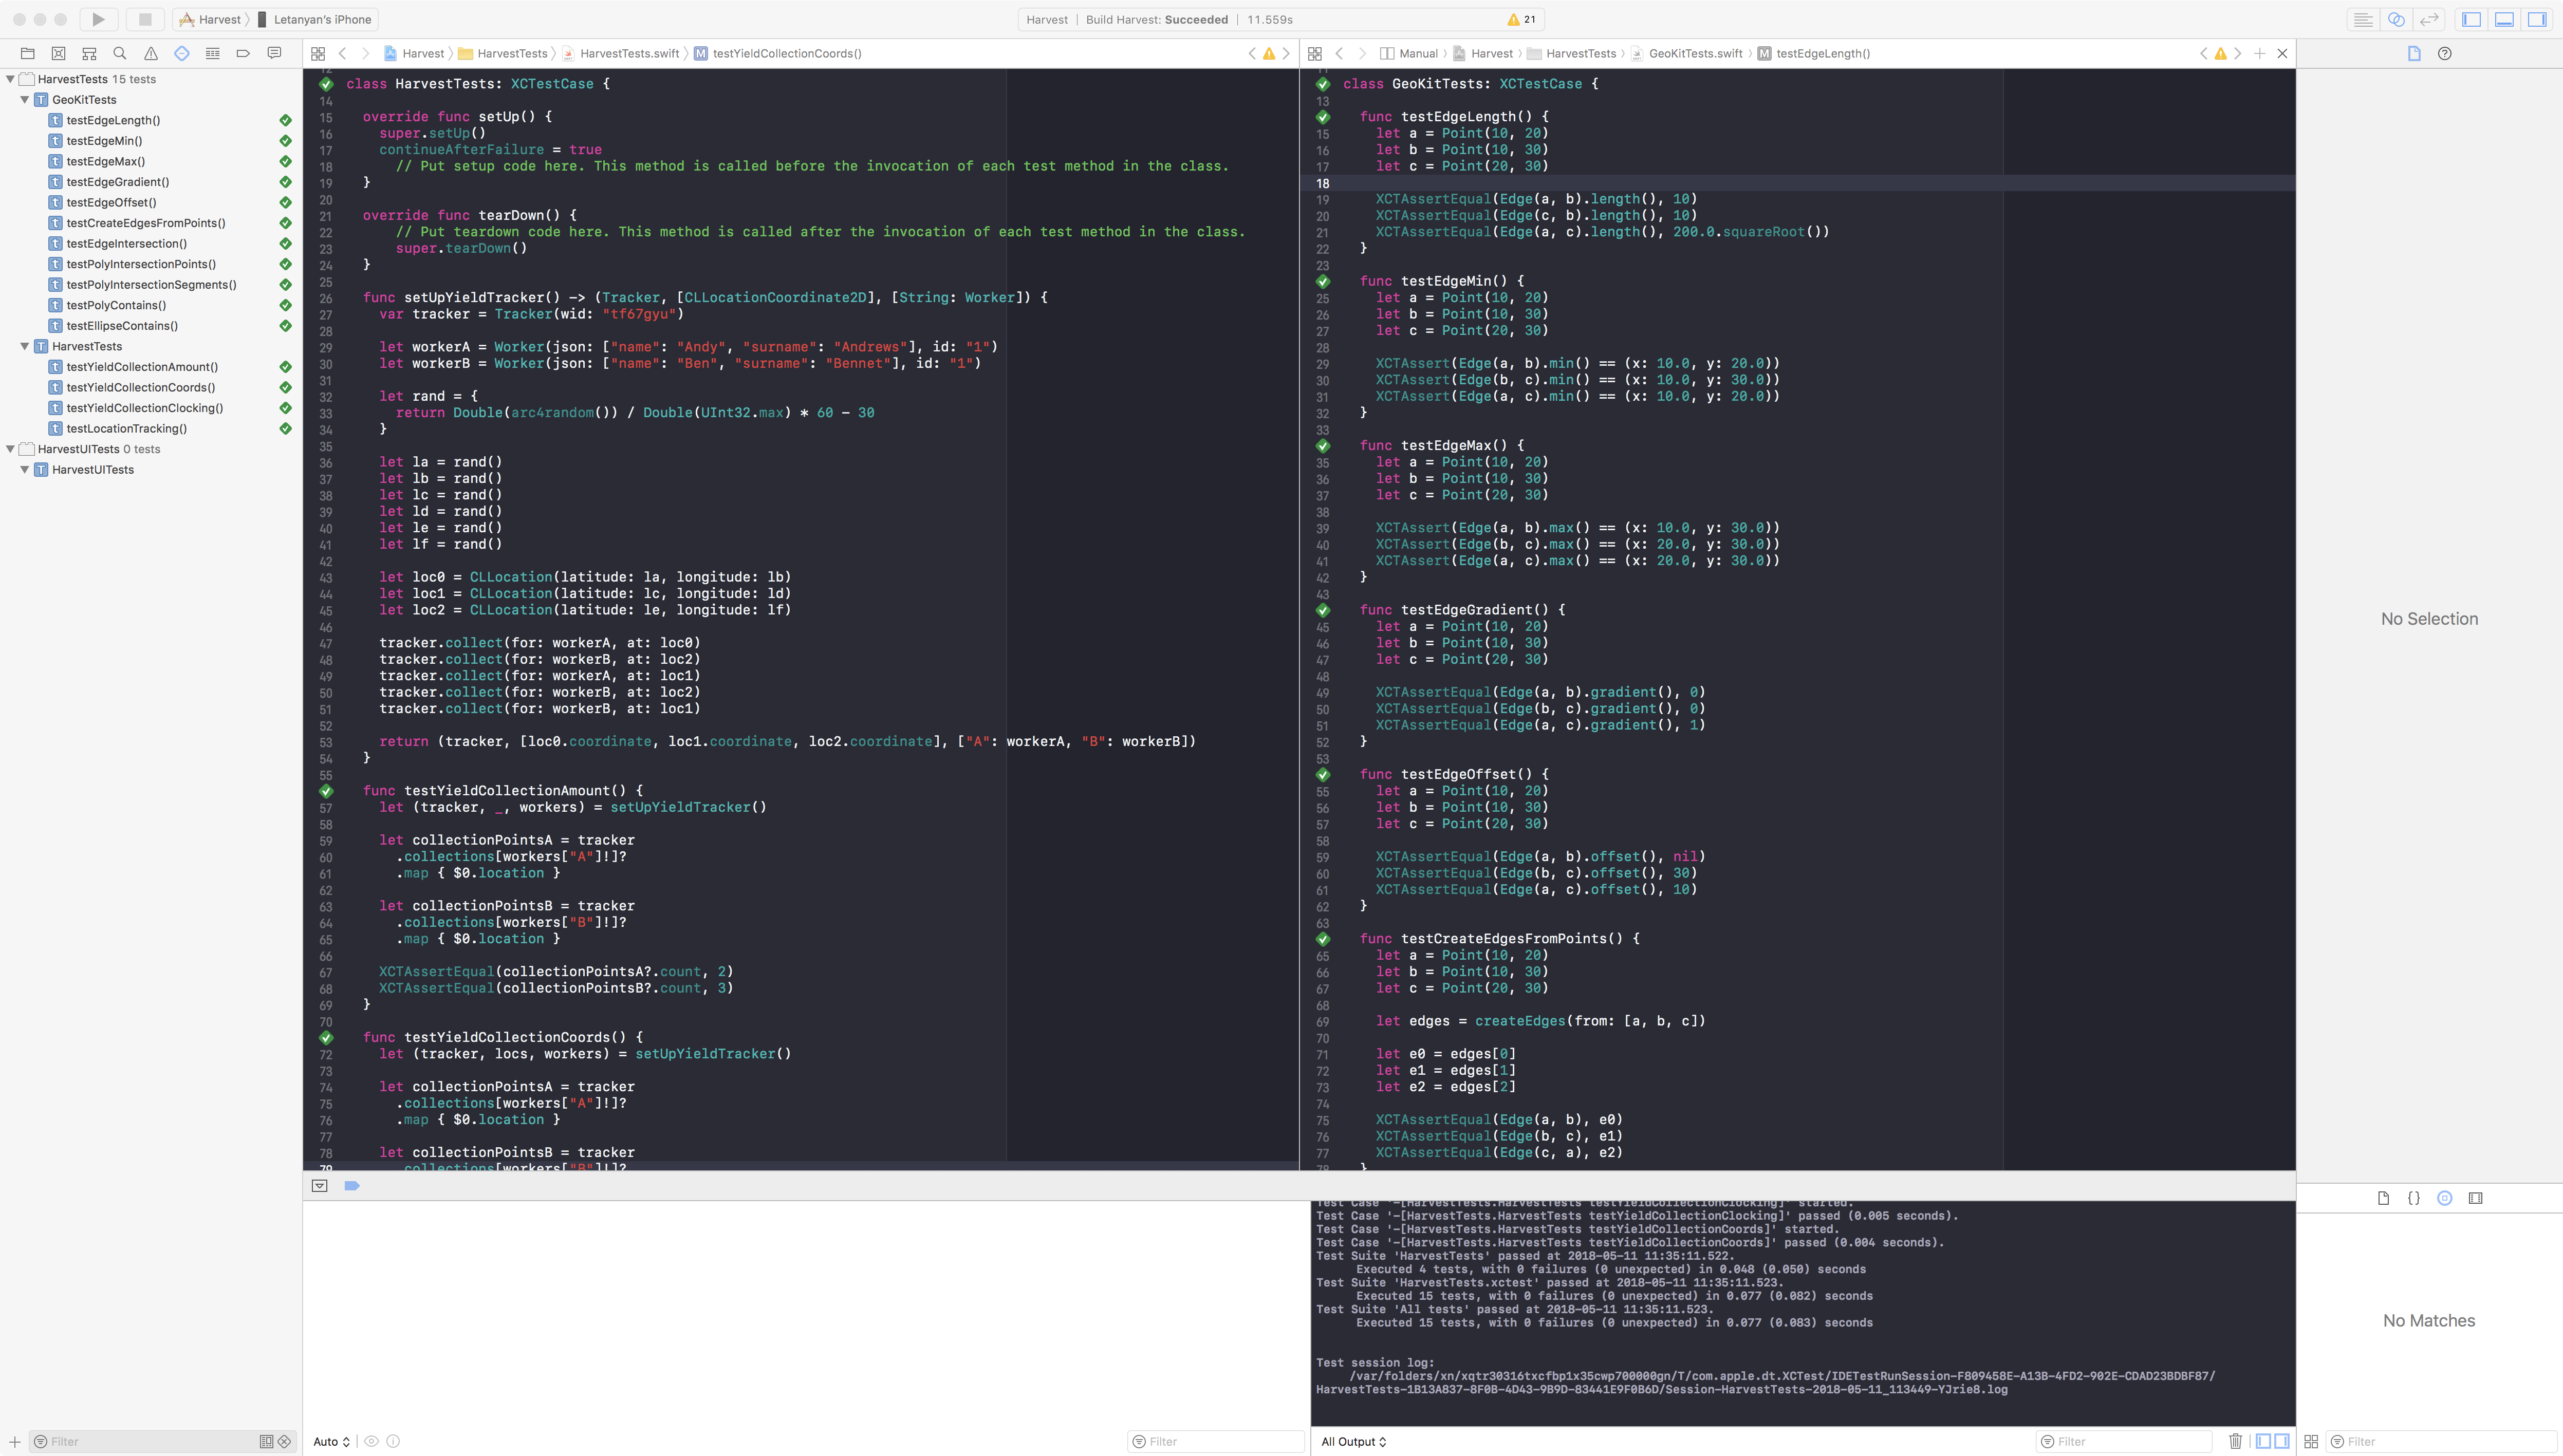
\includegraphics[width=400px]{images/iostest}
\href{https://github.com/BinaryNinjaz/COS301-Capstone/tree/master/Source/iOS/Harvest/HarvestTests}{Link to IOS App Testing}
\newline

  \subsection{NPM}
  The Ava framework will be used for automated testing purposes. To run tests one will need to run "npm test" from the testing directory.
  \subsection{XCode}
  The XCTest framework will be used for out automated testing purposes. To run tests one will need XCode. To execute the tests one will need to use XCodes build command.
 
  \section{TESTING PHILOSOPHY}
  Implementation of both simple and holistic tests will be of concern. However, holistic testing will be of more interest. Testing workflows are of vital importance. The project does not have many simple tasks that could provide us with the safety guarantees we would like. We instead seek to find safety in implementing tests that check the whole interaction of these few unit cases.
  
  \subsection{Benefits}
  Automated test provide developers with the ability to have safe of mind that they have not made any changes that break the program in any way or introduce bugs in any part of the program.
  Forcing developers to write tests forces them to check every part of code they write making tests a form of documentation of a projects requirements.
  
  \section{TEST EVALUATION}
  Strict zero test case failure will be followed. Any branch with a failing test case will never be merged into master. Hence we will ensure that every branch runs tests before a pull request.
  
\end{document}
